\section{Generalised gamma convolutions and the Thorin condition}\label{ch:ggc}

The Thorin condition on the clock $1/G$, equivalent to RH by Proposition~\ref{prop:rigid}, is that it be the Laplace transform of a generalised gamma convolution.

\subsection{The definition and its three readings}\label{sec:ch3:readings}

As in Section~\ref{ch:clock}, a random variable $H\ge0$, or its law, is a generalised gamma convolution (GGC) if
\begin{equation}\label{eq:ch3:ggc}
\E e^{-uH}=\exp\Big\{-du-\int_{(0,\infty)}\log\Big(1+\frac uz\Big)U(dz)\Big\},\qquad u>0,
\end{equation}
with drift $d\ge0$ and a positive Radon measure $U$ on $(0,\infty)$, the Thorin measure, such that $\int_{(0,1)}|\log z|\,U(dz)+\int_{(1,\infty)}z^{-1}U(dz)<\infty$ \cite{Thorin77a,Thorin}, \cite[p.~29]{Bondesson}. The drift and the Thorin measure are unique \cite[p.~30]{Bondesson}. Since $\log(1+u/z)$ is the Laplace exponent of the exponential law with rate $z$, a discrete measure $U=\sum_jc_j\delta_{z_j}$ makes $H$ the sum of $d$ and independent gamma variables with shapes $c_j$ and rates $z_j$. The class is the closure of such sums under weak limits (Thorin's closure theorem, Section~\ref{sec:weak:limits}).

The first reading is through the L\'evy measure. Frullani's integral $\log(1+u/z)=\int_0^\infty(1-e^{-ut})e^{-zt}t^{-1}dt$ turns \eqref{eq:ch3:ggc} into
\[
-\log\E e^{-uH}=du+\int_0^\infty\big(1-e^{-ut}\big)\frac{k(t)}t\,dt,\qquad k(t)=\int e^{-zt}\,U(dz),
\]
so $H$ is infinitely divisible with L\'evy density $k(t)/t$, and its canonical function $k$, $t$ times the L\'evy density, is completely monotone. Conversely, by Bernstein's theorem, an infinitely divisible law on $[0,\infty)$ with drift $d$ and L\'evy density $k(t)/t$, $k$ completely monotone, is a GGC whose Thorin measure is the measure representing $k$ \cite[Section 1.2]{JRY}. For the clock, the unconditional formula for $\log G$ in Section~\ref{ch:clock} gives $k=W$, the heat trace, so the Thorin condition is the complete monotonicity of $W$.

The second reading is through the Stieltjes transform of the Thorin measure. Differentiating the logarithm of \eqref{eq:ch3:ggc} gives
\[
f_H(u)=-\frac{d}{du}\log\E e^{-uH}=d+\int\frac{U(dz)}{u+z},
\]
a nonnegative constant plus the Stieltjes transform of a positive measure, holomorphic on $\cut$. At distance $\eta>0$ below the cut, $\pi^{-1}\im f_H(-x-i\eta)=\int P_\eta(x-z)\,U(dz)$ is the Poisson smoothing of $U$, with $P_\eta$ the Poisson kernel of Section~\ref{ch:clock}, and letting $\eta\downarrow0$ recovers $U$ by Stieltjes inversion: for continuity points $a<b$ of $U$,
\begin{equation}\label{eq:ch3:inversion}
U\big((a,b]\big)=\lim_{\eta\downarrow0}\frac1\pi\int_a^b\im f_H(-x-i\eta)\,dx.
\end{equation}

For the clock, $G'/G=-\frac d{du}\log(1/G)$ takes the place of $f_H$ whether or not RH holds. The chain rule applied to $G(s^2)=\xi(\frac12+s)/\xi(\frac12)$ gives $(\xi'/\xi)(\frac12+s)=2s\,(G'/G)(s^2)$. At $s=\varepsilon+i\theta$ we have $\bar s^2=-x-i\eta$ with $x=\theta^2-\varepsilon^2$ and $\eta=2\varepsilon\theta$, and since $G$ is real on the real axis, \eqref{eq:rho} becomes
\[
\rho_\varepsilon(\theta)=2\theta\cdot\frac1\pi\im\frac{G'}{G}(-x-i\eta)+\frac{2\varepsilon}\pi\re\frac{G'}{G}(s^2).
\]
The first term is the integrand of \eqref{eq:ch3:inversion} at distance $\eta=2\varepsilon\theta$ from the cut, multiplied by the Jacobian $dx/d\theta=2\theta$; the second carries the factor $\varepsilon$. The Thorin density at resolution $\varepsilon$ is therefore a regularised Stieltjes inversion, taken along the parabola $u=(\varepsilon-i\theta)^2$ rather than along a horizontal line.

Under RH the logarithm gives the counting function directly: for $y>0$ not of the form $\gamma^2$, $U_{\RH}((0,y])=-\pi^{-1}\im\log G(-y-i0)=N(\sqrt y)$, with $\log G$ continued from $(0,\infty)$ through the lower half plane, since the factor $1+u/\gamma^2$ of $G$ has argument $-\pi$ at $u=-y-i0$ when $\gamma^2<y$ and $0$ otherwise.

The third reading is as a product. If $U=\sum_jc_j\delta_{z_j}$ is discrete, \eqref{eq:ch3:ggc} is the product $e^{-du}\prod_j(1+u/z_j)^{-c_j}$ of gamma Laplace transforms. Conversely, if $F$ is entire of genus zero with $F(0)=1$ and all its zeros real and negative, then $1/F$ is the Laplace transform of a GGC with $d=0$ and a unit atom at $-u_j$ for each zero $u_j$ of $F$, counted with multiplicity. For the clock $F=G$, the product is Hadamard's \eqref{eq:ch2:hadamard}, and the Thorin condition says that every zero $-a_k$ of $G$ is real and negative, that is, $a_k>0$.

\subsection{The Bondesson hierarchy and the clock}\label{sec:ch3:hierarchy}

Between the infinitely divisible laws on $[0,\infty)$ (ID) and the GGCs lie two classes defined by conditions on the L\'evy density $k(t)/t$: the self decomposable laws (SD), for which $k$ is nonincreasing, and the Bondesson class (BO), for which $k(t)/t$ is completely monotone. The GGCs are the laws for which $k$ itself is completely monotone, and inside them lie the laws with a hyperbolically completely monotone density (HCM, defined below). The inclusions are
\[
\mathrm{HCM}\subset\mathrm{GGC}\subset\mathrm{SD}\subset\mathrm{ID},\qquad \mathrm{GGC}\subset\mathrm{BO}\subset\mathrm{ID},
\]
and SD and BO are not nested. The L\'evy density $e^{-t}(1+\frac1{2t})$ is completely monotone, but $k(t)=e^{-t}(t+\frac12)$ increases on $(0,\frac12)$, so the law is in BO and not in SD \cite[Section 2]{P17}; the L\'evy density $t^{-1}\mathbf 1_{t<1}$ gives a law in SD and not in BO, since a completely monotone function that vanishes on $(1,\infty)$ vanishes identically.

A positive continuous function $\varphi$ on $(0,\infty)$ is hyperbolically completely monotone if for every $u>0$ the function $\varphi(uv)\varphi(u/v)$ is completely monotone in $w=v+v^{-1}$, and a law is HCM if it has an HCM density. By Bondesson's theorem \cite[Theorem 6.1.1]{Bondesson}, a function $\varphi$ with $\varphi(0+)=1$ is the Laplace transform of a GGC if and only if it is HCM, so the Thorin condition becomes a family of sign conditions on real derivatives. An HCM law is a GGC, so the HCM property of a law is stronger than that of its Laplace transform, and strictly so: the GGC of Theorem~\ref{bs:thm:eta} has an HCM Laplace transform and a density that is not HCM.

\begin{resultpar}
The extended generalised gamma convolutions (EGGC), introduced by Thorin \cite{Thorin78}, are the weak limits of convolutions of gamma laws and their reflections \cite[Section 7.1]{Bondesson}. A symmetric law is an EGGC if and only if it is the law of $Z\sqrt{2H}$ with $Z$ standard normal and $H$ an independent GGC \cite[Theorem 7.3.1]{Bondesson}. Since $\E e^{i\theta Z\sqrt{2T}}=\E e^{-\theta^2T}$ determines the law of $T$, the variable $Z\sqrt{2T}$ of the van Dantzig pair of Section~\ref{ch:clock} is an EGGC if and only if $T$ is a GGC, that is, by Proposition~\ref{prop:rigid}, if and only if RH holds. With no hypothesis $Z\sqrt{2T}$ is self decomposable: subordinating the L\'evy measure $W(v)\,dv/v$ of $T$ to the heat kernel gives the L\'evy density $k(|x|)/|x|$ with $k(r)=\int_0^\infty e^{-1/4v}(4\pi v)^{-1/2}W(r^2v)\,dv/v=\sum_je^{-r\sqrt{a_j}}$ (the first passage identity for each term, with the principal root), and $k$ decreases because $W$ does (Theorem~\ref{thm:ch12:idsd}).\label{tx3:res:sdz} The $z$ distributions of Barndorff-Nielsen, Kent and S{\o}rensen \cite{BNKS82} are the lattice analogue of this family of variance mixtures.
\end{resultpar}

Table~\ref{tab:ch3:hierarchy} records what is known about the sign conditions on $W$ that the classes become for the clock. Section~\ref{ch:finite} explains why no finite number of derivative conditions can reach the last row.

\begin{table}[htbp]
\centering\small
\begin{tabular}{p{0.24\textwidth}p{0.32\textwidth}p{0.34\textwidth}}
\toprule
class or property & condition on $W$ & status for the clock\\
\midrule
ID & $W\ge0$ & \raggedright proved, with the zeros verified to height $1000$ (Theorem~\ref{thm:ch12:idsd})\tabularnewline
SD & $W$ nonincreasing & \raggedright proved, with the zeros verified to height $1000$ (Theorem~\ref{thm:ch12:idsd})\tabularnewline
strict log convexity & \raggedright ${WW''>W'^2}$ and ${W'W'''>W''^2}$ & \raggedright proved, with the zeros verified to height $1000$ (Section~\ref{ch:heat})\tabularnewline
\raggedright derivative signs to order $1.16\times10^{25}$ & $(-1)^nW^{(n)}>0$ for $n\le1.16\times10^{25}$ & \raggedright proved, with the zeros verified to height $3\times10^{12}$ (Theorem~\ref{thm:ch12:window})\tabularnewline
\raggedright complete monotonicity near the origin & $(-1)^nW^{(n)}(t)>0$ for every $n$ and $t\le1.29$ & \raggedright proved, with the zeros verified to height $10^{12}$ (Theorem~\ref{thm:ch12:cmint})\tabularnewline
BO & $W(t)/t$ completely monotone & \raggedright equivalent to RH (Section~\ref{sec:ch16:max}); open\tabularnewline
GGC & $W$ completely monotone & equivalent to RH; open\\
\bottomrule
\end{tabular}
\caption{The Bondesson hierarchy on the clock, whose L\'evy density is $W(t)/t$.}
\label{tab:ch3:hierarchy}
\end{table}

Urbanik's classes of multiply self decomposable laws give conditions on $W$ of another kind: with $L_0$ the class of self decomposable laws and $L_n$ that of the self decomposable laws whose driving process has its law in $L_{n-1}$, the clock lies in $L_n$ exactly when $(-t\frac d{dt})^jW\ge0$ for $j\le n+1$ (Section~\ref{pk:sec:ladder}), and for $n\ge1$ this does not follow from the GGC property, since the exponential law is a GGC whose canonical function $e^{-t}$ has $(-t\frac d{dt})^2e^{-t}=-t(1-t)e^{-t}<0$ for $t<1$. For the clock these conditions hold for $n=2$ and fail for $n=3$, with no hypothesis (Theorem~\ref{pk:thm:ladder}), while membership of every $L_n$ would imply RH, since $\bigcap_nL_n$ lies inside the GGCs \cite{BergForst83}.

\subsection{Diagnostics for the Thorin condition}\label{sec:ch3:diag}

RH can be stated as a GGC identity on a real interval. The right side of \eqref{eq:ch3:ggc} extends to a holomorphic nonvanishing function on $\cut$ (Exercise~\ref{ex:ch3:cont}), so RH holds if and only if there is a GGC $H$ with $\xi(\frac12)/\xi(\frac12+s)=\E e^{-s^2H}$ for real $0<s<1$ alone \cite[Proposition 3.3]{P17}.

As it stands the identity is of no use to a computation, because analytic continuation from an interval is unstable. A unit Thorin atom at $z_0$ multiplies the transform by $(1+u/z_0)^{-1}$, which differs from one by less than $1/z_0$ on $(0,1)$, so transforms that agree to high accuracy on $(0,1)$ can have very different Thorin measures at large $z$. Riesz's criterion meets the same obstruction: its numbers $1/\zeta(2k)$ are, up to explicit factors, values of the clock at the real points $(2k-\frac12)^2$, and they bear on the zeros only through the analytic interpolation of $k\mapsto1/\zeta(2k)$ into the strip $\frac14<\re k<\frac12$ (Section~\ref{ri:sec:help}). The information about the zeros enters through the analyticity that the representation forces, and a computation has to supply it in another way: through values of $\xi$ and $\xi'$ at complex arguments, which Chapter~\ref{chap:evaluation} computes, or through sign conditions on derivatives of every order. Each characterisation of Sections~\ref{sec:ch3:readings} and \ref{sec:ch3:hierarchy} yields such a test, and Table~\ref{tab:ch3:diag} lists them with what a failure proves.

\begin{table}[htbp]
\centering\small
\begin{tabular}{p{0.19\textwidth}p{0.37\textwidth}p{0.34\textwidth}}
\toprule
diagnostic & computes & a failure proves\\
\midrule
pole test & poles of $G'/G$ off $(-\infty,0]$ & \raggedright not GGC; for the clock, a zero off the line\tabularnewline
\raggedright Thorin density at resolution $\varepsilon$ & $\rho_\varepsilon=\pi^{-1}\re(\xi'/\xi)$ at $\frac12+\varepsilon+i\theta$ & \raggedright a zero with $\re\rho>\frac12+\varepsilon$ (Proposition~\ref{prop:struct}, \cite{Lagarias})\tabularnewline
zero density scan & \raggedright $M_\varepsilon(T)+\tau_\varepsilon(T)$ against $N(T)$ (Proposition~\ref{prop:zerodensity}) & \raggedright ${\frac12[N(T)-M_\varepsilon(T)-\tau_\varepsilon(T)]}$ zeros with $\re\rho>\frac12+\varepsilon$ below height $T$\tabularnewline
heat trace signs & $(-1)^nW^{(n)}(t)$ & \raggedright not GGC; finitely many orders are consistent with off line zeros (Section~\ref{ch:finite})\tabularnewline
Hankel blocks & $\det[(-1)^{i+j}W^{(i+j)}(t)]$ & \raggedright not GGC (Weil's criterion at one scale, Section~\ref{ch:heat})\tabularnewline
HCM test & $(-1)^n\partial_w^n[\varphi(uv)\varphi(u/v)]$ & not GGC (Section~\ref{ch:weak})\\
Bernstein test & $(-1)^{n-1}L^{(n)}$, $L=\log G$ & \raggedright not ID, which Theorem~\ref{thm:ch12:idsd} excludes for the clock\tabularnewline
Stieltjes moments & \raggedright Hankel matrices $[m_{i+j}]$ and $[m_{i+j+1}]$, $m_n=\sum_ka_k^{-n-1}$ & not GGC\\
\bottomrule
\end{tabular}
\caption{Diagnostics for the Thorin condition. The pole test, the Thorin density and the zero density scan locate a failure in height; the others detect it only globally.}
\label{tab:ch3:diag}
\end{table}

The diagnostics differ in how strongly they weight the higher zeros. Those built from $W$ see a zero at height $\gamma$ through $e^{-\gamma^2t}$: in $(-1)^nW^{(n)}(t)=\sum_ja_j^ne^{-a_jt}$ it enters with weight $(\gamma/\gamma_1)^{2n}e^{-(\gamma^2-\gamma_1^2)t}$ relative to the first zero. These tests certify easily and discriminate poorly. The Bernstein test on $L(u)=\log G(u)$, computed for $u>\frac14$, where the Dirichlet series of $\log\zeta(\frac12+\sqrt u)$ converges, is better conditioned \cite[Section 18.2.2]{P26}: since $(-1)^{n-1}L^{(n)}(u)=(n-1)!\sum_k(u+a_k)^{-n}$, a zero at height $\gamma$ enters with relative weight of order $(\gamma_1/\gamma)^{2n}$. It too sees the higher zeros only through subdominant terms, and for the clock it cannot fail: by the formula for $\log G$ in Section~\ref{ch:clock}, $(-1)^{n-1}L^{(n)}(u)=\int_0^\infty t^{n-1}e^{-ut}W(t)\,dt$, which is positive because $W>0$ (Theorem~\ref{thm:ch12:idsd}). Read at $u=0$ through \eqref{eq:ch2:mgf}, which gives $\log\E e^{hX}=\log G(h^2)$, the same formula makes the even cumulants of the P\'olya variable $X$ alternate in sign with no hypothesis: $(-1)^{n-1}\kappa_{2n}(X)=\frac{(2n)!}{n!}\int_0^\infty t^{n-1}W(t)\,dt>0$ for every $n\ge1$. Under RH this is the sign rule that Newman proved for laws of Lee Yang type \cite{Newman75}. Complete monotonicity of $L'$ is weaker than the Thorin condition, which asks that $L'$ be the Stieltjes transform $\int U(dz)/(u+z)$ of a positive measure $U$.

The Thorin density and the zero density scan built from it are local in the ordinate without a search for zeros: by Proposition~\ref{prop:struct}, a zero at height $\gamma$ contributes about $1/(\pi\varepsilon)$ to $\rho_\varepsilon$ at $\theta=\gamma$ and about $\varepsilon/(\pi d^2)$ at distance $d\gg\varepsilon$.

\subsection{Explicit Thorin measures and the sinh benchmark}\label{sec:ch3:bench}

Table~\ref{tab:ch3:cat} lists GGCs whose Thorin measures are explicit, in the variable $u$ of the clock. They are models for the clock, test cases for code, and the building blocks of the Vere-Jones representation of Section~\ref{ch:rz1} (Theorem~\ref{rz:thm:saw} and Table~\ref{rz:tab:measures}).

\begin{table}[htbp]
\centering\small
\begin{tabular}{p{0.31\textwidth}p{0.33\textwidth}p{0.26\textwidth}}
\toprule
Laplace transform & Thorin measure & law\\
\midrule
$(1+u/z_0)^{-a}$ & $a\,\delta_{z_0}$ & $\mathrm{Gamma}(a,z_0)$\\
$\pi\sqrt u/\sinh(\pi\sqrt u)$ & $\sum_{k\ge1}\delta_{k^2}$ & $2K^2$, $K$ Kolmogorov\\
$(\sqrt u/\sinh\sqrt u)^2$ & $2\sum_{k\ge1}\delta_{\pi^2k^2}$ & $S_2/2$ (Williams)\\
$\sech\sqrt u$ & $\sum_{k\ge1}\delta_{(k-\frac12)^2\pi^2}$ & \raggedright exit time of $\sqrt2B$ from $(-1,1)$\tabularnewline
$(\sech\sqrt u)^{1/2}$ & $\frac12\sum_{k\ge1}\delta_{(k-\frac12)^2\pi^2}$ & Meixner time\\
$e^{-c\sqrt u}$ & $c\,(2\pi\sqrt z)^{-1}dz$ & positive stable, index $\frac12$\\
$(1+\sqrt u/c)^{-1}$ & $c\,\{2\pi\sqrt z(z+c^2)\}^{-1}dz$ & $E^2S/c^2$\\
$e^{x(\alpha-\sqrt{\alpha^2+2u})}$ & $x\{\pi\sqrt{2z-\alpha^2}\}^{-1}\mathbf 1_{z>\alpha^2/2}dz$ & inverse Gaussian\\
$\exp\{1-x\sqrt u-e^{-x\sqrt u}\}$ & $x\sin^2(x\sqrt z/2)(\pi\sqrt z)^{-1}dz$ & \raggedright one compensated jump, by \eqref{eq:sin2}\tabularnewline
$\mathcal W(u)/u$ & \raggedright image of $db/\pi$ on $(0,\pi)$ under $r(b)=b\,e^{-b\cot b}/\sin b$ & \raggedright Lambert law (Theorem~\ref{pk:thm:lambert})\tabularnewline
$K_0(2\pi)/K_{\sqrt u}(2\pi)$ & \raggedright $\sum_{n\ge1}\delta_{\nu_n^2}$, $\nu_n$ the zeros of $\nu\mapsto K_{i\nu}(2\pi)$ & \raggedright hitting time of a diffusion (Theorem~\ref{thm:biane:clock})\tabularnewline
$\xi(\alpha)/\xi(\alpha+\sqrt u)$, $\alpha\ge1$ & $v_\alpha(\sqrt z)(2\pi\sqrt z)^{-1}dz$ & \raggedright shifted clock (Theorem~\ref{thm:poisson})\tabularnewline
$\xi(\frac12)/\xi(\frac12+\sqrt u)$ & \raggedright $\sum_{\gamma>0}\delta_{\gamma^2}$ if and only if RH holds & \raggedright the clock (Proposition~\ref{prop:rigid})\tabularnewline
\bottomrule
\end{tabular}
\caption{GGC Laplace transforms in the variable $u$, their Thorin measures in $z$, and the corresponding laws.}
\label{tab:ch3:cat}
\end{table}

In the table, $K$ is the Kolmogorov variable; $S_2$ is as in Section~\ref{ch:clock}; $B$ is a standard Brownian motion; the Meixner time $H$ has $\E e^{-uH}=(\sech\sqrt u)^{1/2}$, so that $Z\sqrt{2H}$, with $Z$ standard normal and independent of $H$, has the Meixner law of Section~\ref{ch:rz2}, whose time in Proposition~\ref{rz:prop:meixstruct} is $2H$; and $S$ is the positive stable variable with $\E e^{-uS}=e^{-\sqrt u}$, independent of the standard exponential variable $E$. Rows two to five are the classical hyperbolic laws \cite{BPY01}. At $u=-t^2$ the reciprocals of rows two and four become $\sin(\pi t)/(\pi t)$ and $\cos t$, the characteristic functions of the uniform law on $(-\pi,\pi)$ and of a symmetric sign. Like $\Xi$, both have infinitely many real zeros, so real zeros do not obstruct the Thorin property; the property requires them. For the clock, unlike these models, the positivity of the points $a_k$ is the conclusion to be proved \cite[Section 10]{P17}.

The sinh clock $1/G_0$, with $G_0(u)=\sinh(\pi\sqrt u)/(\pi\sqrt u)=\prod_{k\ge1}(1+u/k^2)$, is the second row of the table. It has the structure that the clock has under RH, a GGC with unit Thorin atoms, but its ordinates are the integers, equally spaced, and no arithmetic enters. Its Thorin density at resolution $\varepsilon$, the density in $\theta=\sqrt z$ of a measure $\mu^{(0)}_\varepsilon$, is
\[
\rho^{(0)}_\varepsilon(\theta)=\frac1\pi\re\Big[\pi\coth\big(\pi(\varepsilon+i\theta)\big)-\frac1{\varepsilon+i\theta}\Big]=\sum_{k\ne0}P_\varepsilon(\theta-k),
\]
exactly the Poisson smoothing of the atoms and their reflections, so the matched total variation of Section~\ref{ch:distances} vanishes identically. The cumulative mass is explicit. As for $\xi$ (Section~\ref{ch:distances}), it is $\pi^{-1}$ times the change in the argument of $\sinh(\pi s)/(\pi s)$ along $s=\varepsilon+i\theta$, and at a half integer $\Theta=m+\frac12$ the continuous argument of $\sinh(\pi(\varepsilon+i\theta))$ has grown from $0$ to $\pi\Theta$ and that of $\varepsilon+i\theta$ to $\frac\pi2-\arctan(\varepsilon/\Theta)$, so that
\[
\mu^{(0)}_\varepsilon\big((0,\Theta^2]\big)=m+\frac1\pi\arctan\frac\varepsilon\Theta .
\]
The mass defect $\mu^{(0)}_\varepsilon((0,\Theta^2])-m$ is therefore $\varepsilon/(\pi\Theta)+O(\varepsilon^3)$. On the window $0<\theta\le50.5$, which holds $50$ atoms, the defect is $0.00630\,\varepsilon$ to first order and $3.151\times10^{-3}$ at $\varepsilon=0.5$.

The cell distance, the sum over the cells $C$ of $|\mu^{(0)}_\varepsilon(C)-1|$ as in Section~\ref{ch:distances}, is explicit as well. We use the cells $(k-\frac12,k+\frac12]$, $k=1,\dots,50$, and add the mass of the strip $(0,\frac12]$, which lies in no cell, as unmatched. For the full lattice $\mathbb Z$ each cell would have mass exactly one. The sinh clock lacks the atom at $0$, so each of its cells is short by the mass that $P_\varepsilon$ puts there, and the strip carries $\pi^{-1}\arctan2\varepsilon$; Section~\ref{ch:spacing} computes these masses. Summing,
\[
d^{(0)}_{\rm cell}(\varepsilon)=\frac1\pi\Big[2\arctan2\varepsilon-\arctan\frac\varepsilon{50.5}\Big]=\frac{4-1/50.5}\pi\,\varepsilon+O(\varepsilon^3),
\]
which is $0.4968$, $0.1250$, $0.0631$, $0.01267$ and $0.00633$ at $\varepsilon=0.5$, $0.1$, $0.05$, $0.01$ and $0.005$, and $1.267\,\varepsilon$ in the limit. All of it is due to the atom missing at $0$.

\begin{figure}[htbp]
\centering
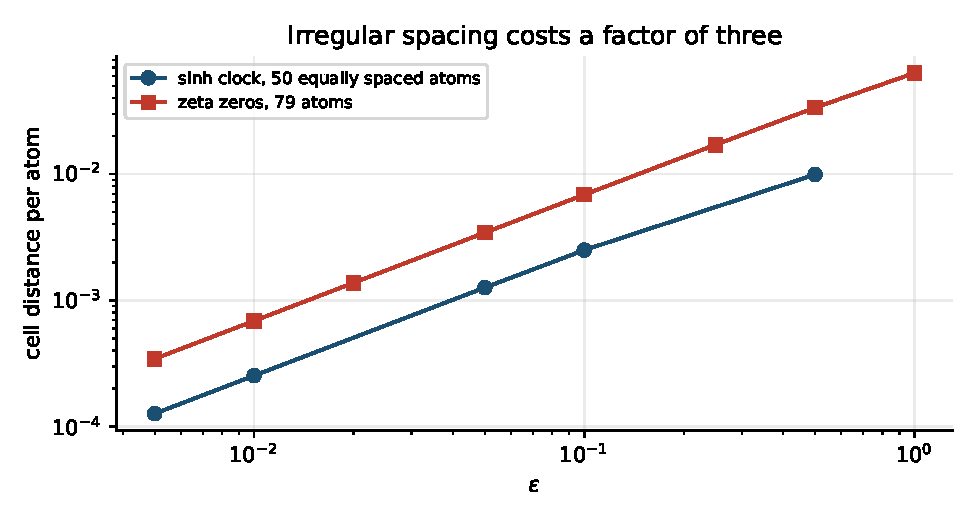
\includegraphics[width=0.72\textwidth]{fig/bench.pdf}
\caption{Cell distance divided by the number of atoms in the window, for the sinh clock ($50$ atoms, cells $(k-\frac12,k+\frac12]$) and for the $79$ zeros below height $200$ (Voronoi cells of Section~\ref{ch:distances}). Both vanish linearly in $\varepsilon$. For the sinh clock the undivided distance stays below $4\varepsilon/\pi$ whatever the number of atoms, so the gap between the curves depends on the window, and the factor of three in the title of the figure holds for these two windows only.}
\label{fig:ch3:bench}
\end{figure}

For the $79$ zeros below height $200$ the constant is $5.44$ (Section~\ref{ch:distances}), and it has a different origin. The zeros are irregularly spaced, so the mass that leaks out of a cell is no longer replaced by the mass that leaks in from its neighbours, and every cell contributes; Section~\ref{ch:spacing} reads the constant as a statistic of the spacings. Figure~\ref{fig:ch3:bench} divides both distances by the number of atoms, which gives $1.267\,\varepsilon/50=0.0253\,\varepsilon$ for the sinh clock and $5.44\,\varepsilon/79=0.069\,\varepsilon$ for the zeros. Their ratio, nearly three, depends on the window, since for the lattice the distance per atom falls like $1/N$ as the window grows to $N$ atoms. Williams' Thorin measure $2\sum_k\delta_{\pi^2k^2}$ of Table~\ref{tab:ch3:cat} needs no separate benchmark: it is the same lattice rescaled by $\pi$, with atoms of mass two, so its Thorin density at resolution $\varepsilon$ is $\frac2\pi\rho^{(0)}_{\varepsilon/\pi}(\theta/\pi)$ and its distances follow by scaling from the closed forms for the sinh clock.

